\documentclass[isoft]{ufgtexposter}

\usepackage{lipsum}
\usepackage{natbib}
\usepackage{booktabs}
\usepackage{subfig} 
\usepackage{amsmath} 
\usepackage{textcomp} 
\usepackage{url}  
\usepackage[hidelinks]{hyperref}
\usepackage[utf8]{inputenc}
\usepackage[portuguese]{babel}
\usepackage{graphicx}
%%%%%%%%%%%%%%%%%%%%%%%%%%%%%%%%%%%%%%%%%
%%               Configs               %%
%%%%%%%%%%%%%%%%%%%%%%%%%%%%%%%%%%%%%%%%%

% Choose one of the section color {ufglhblue | ufgdkblue | dkblue | black | gold}
\setsectioncolor{dkblue} 

% Define width of the rule or hide it by setting 0pt or commenting the command 
\setcolumnseprule{3pt}

% Inform the paths to the logo files or leave empty one or both parameters. 
% There are three options [ T | M | B ] to positioning them.

\setlogos[T]{images/logo}{images/LOGO LAB}

% Choose one of the background options {1 | 2 | 3}. 
% Actually, one can select any graphic file in backgrounds directory. 
\setbackground{3}

% Resize the title to keep it in two lines // {font size}{line height}
\settitlesize{64pt}{68pt}

% Resize the font of the content. Default {32pt}{38pt} // {font size}{line height}
\setcontentfontesize{33pt}{34pt}

% Resize the font of the emails. Default {26pt}{32pt} // {font size}{line height}
\setemailfontesize{42pt}{40pt}

% General info
\title{\uppercase{Coloque aqui seu texto\\<-observe o plular linha
}} 

\author{Primeiro Autor, Segundo Autor e Terceiro Autor} 

\department{Escola Politécnica - USP - Engenharia XXXXXXXX}

\email{ \text{primeiroautor@usp.br, segundoautor@usp.br, terceiroautor@usp.br} }

\class{}

\posteryear{2024}

\copyrightholder{2° Congresso do Programa de Pós Graduação em Engenharia Mecânica e Mecatrônica}

%%%%%%%%%%%%%%%%%%%%%%%%%%%%%%%%%%%%%%%%%
%%           End configs               %%
%%%%%%%%%%%%%%%%%%%%%%%%%%%%%%%%%%%%%%%%%

\pagestyle{fancy}
\begin{document}
    \begin{poster}
    %%%%%%%%%%%%%%%%%%%%%%%%%%%%%%%%%%%%%%%%%
    %%             Begin poster            %%
    %%%%%%%%%%%%%%%%%%%%%%%%%%%%%%%%%%%%%%%%%
    
    \section{Introdução}
            \lipsum[3]
        
    \section{Materiais e métodos}%
        
        \subsection{Coloque aqui seu modelo}
        
        \lipsum[11]
        
        \vspace{0.1cm}
        
        \begin{figure}
            \centering
            \captionsetup{type=figure}
            %mude o scale até sua imagem ficar do tamanho certo o scale pode ter valores menores que 
            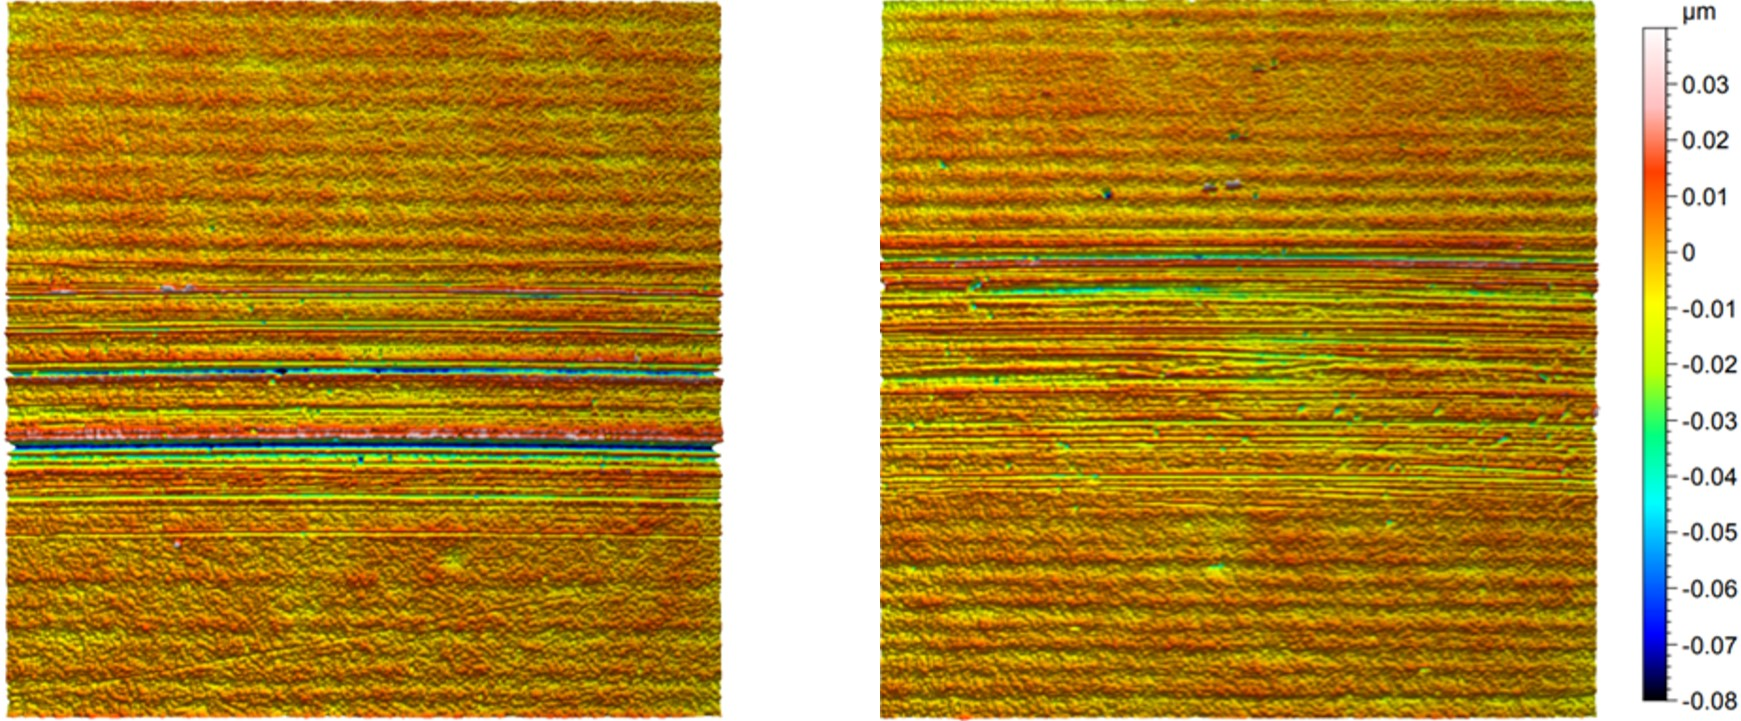
\includegraphics[scale=0.8]{images/exemplo.jpg}
            \caption{Trilha de desgaste topografia}
            \label{fig:lstm}
        \end{figure}
        
        \subsection{Coloque aqui seu \textit{dataset}}
        
            \lipsum[54]
            
            \vspace{0.5cm}
            %Aaqui começa a tabela
            \begin{table}
                \centering
                \captionsetup{type=table}
                \caption{\textit{Corpus} utilizados no estudo}
                \label{Corpus}
                \renewcommand{\arraystretch}{1.2}
                \resizebox{0.47\textwidth}{!}{%
                \begin{tabular}{lcccclcl}
                    \hline
                    &\textbf{Corpus}    &  \textbf{Caracteres únicos} &    &  \textbf{Total de linhas}  &  & \textbf{Total de caracteres} &  \\ \hline
                    &SBSEThesis         & 88  &    &    2.311     &        & 771.179 &  \\ 
                    &Bible              & 63  &    &    32.359   &        & 3.924.374 &  \\
                    &JavaCode           & 69  &    &    436.565  &        & 12.053.424 &  \\ \hline
                \end{tabular}
            }
            \end{table}
            \vspace{0.5cm}
            
            \lipsum[57]
            
            \citep{defects2j}.
    
            \subsection{Subsection}
                \lipsum[8]
    
        \section{Resultados}%
                
            \lipsum[4]    
    
            \begin{figure}
                \centering
                \captionsetup{type=figure}
                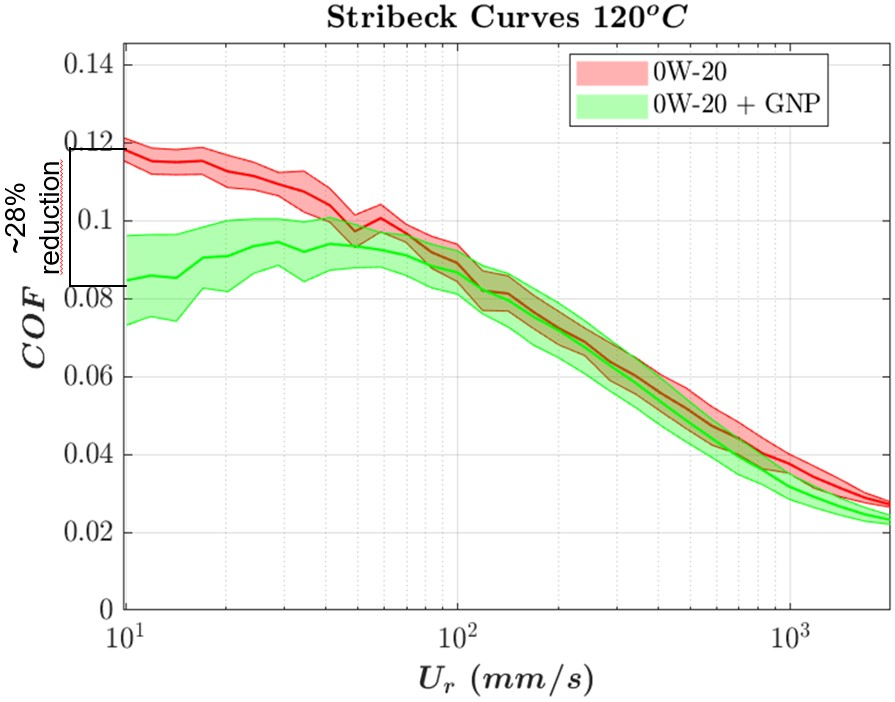
\includegraphics[scale=1.3]{images/curva stribeck.jpg}
                \caption{Curva de stribeck \textit{}.}
                \label{fig:result}
            \end{figure}
    
            \lipsum[5]
            \cite{chollet2015keras}     
    
        \section{Considerações finais}
    
            \lipsum[15]
    
        \section{Agradecimento}
    
            \lipsum[57]
    
        \bibliographystyle{abbrv}
        \bibliography{refs}
    
    %%%%%%%%%%%%%%%%%%%%%%%%%%%%%%%%%%%%%%%%%
    %%               End poster            %%
    %%%%%%%%%%%%%%%%%%%%%%%%%%%%%%%%%%%%%%%%%
    
    \end{poster}

\end{document}

 
